% !TeX root = ../main.tex

\chapter{制造,组装与测试}
\label{cha:chapter03}
\section{制造与组装}
图\ref{fig:CAD}和图\ref{fig:carbon_fiber}为第一版设计的机身碳纤维板设计图和实物。这里遇到的一些小问题是设计时未完全考虑到加工情况,由于开槽是用刀具铣,因此方形的槽是不存在的,角上一定会是半径等于刀具的圆角。这个问题在第三版设计的时候体现得比较明显,不得不对零件进行了手动加工处理才能正常组装。
\begin{figure}[H]
  \centering%
  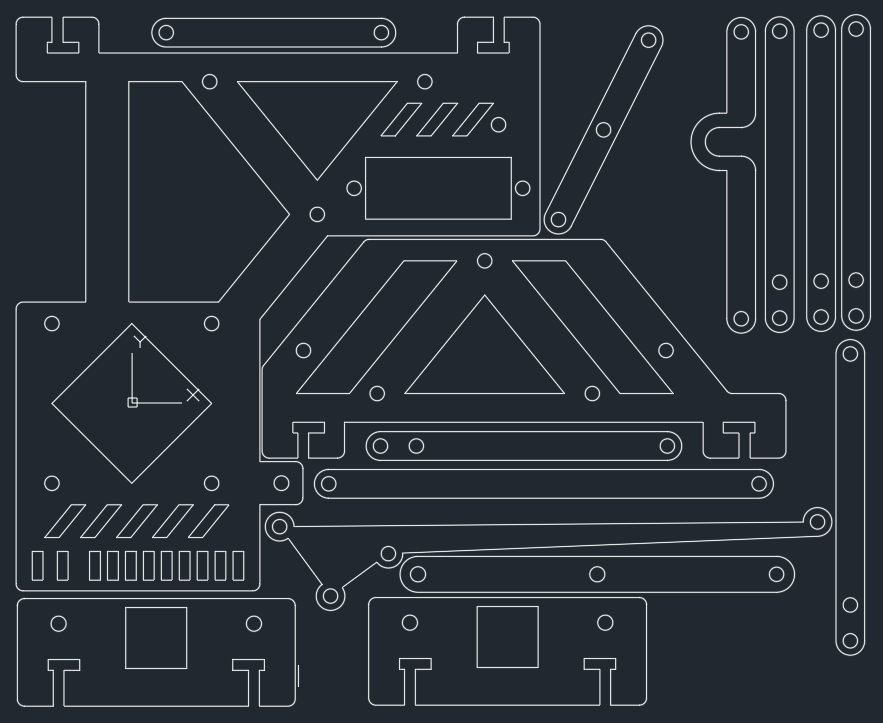
\includegraphics[height=6cm]{CAD.png}
  \caption{CAD设计图(第一版)}
  \label{fig:CAD}
\end{figure}
\begin{figure}[H]
  \centering%
  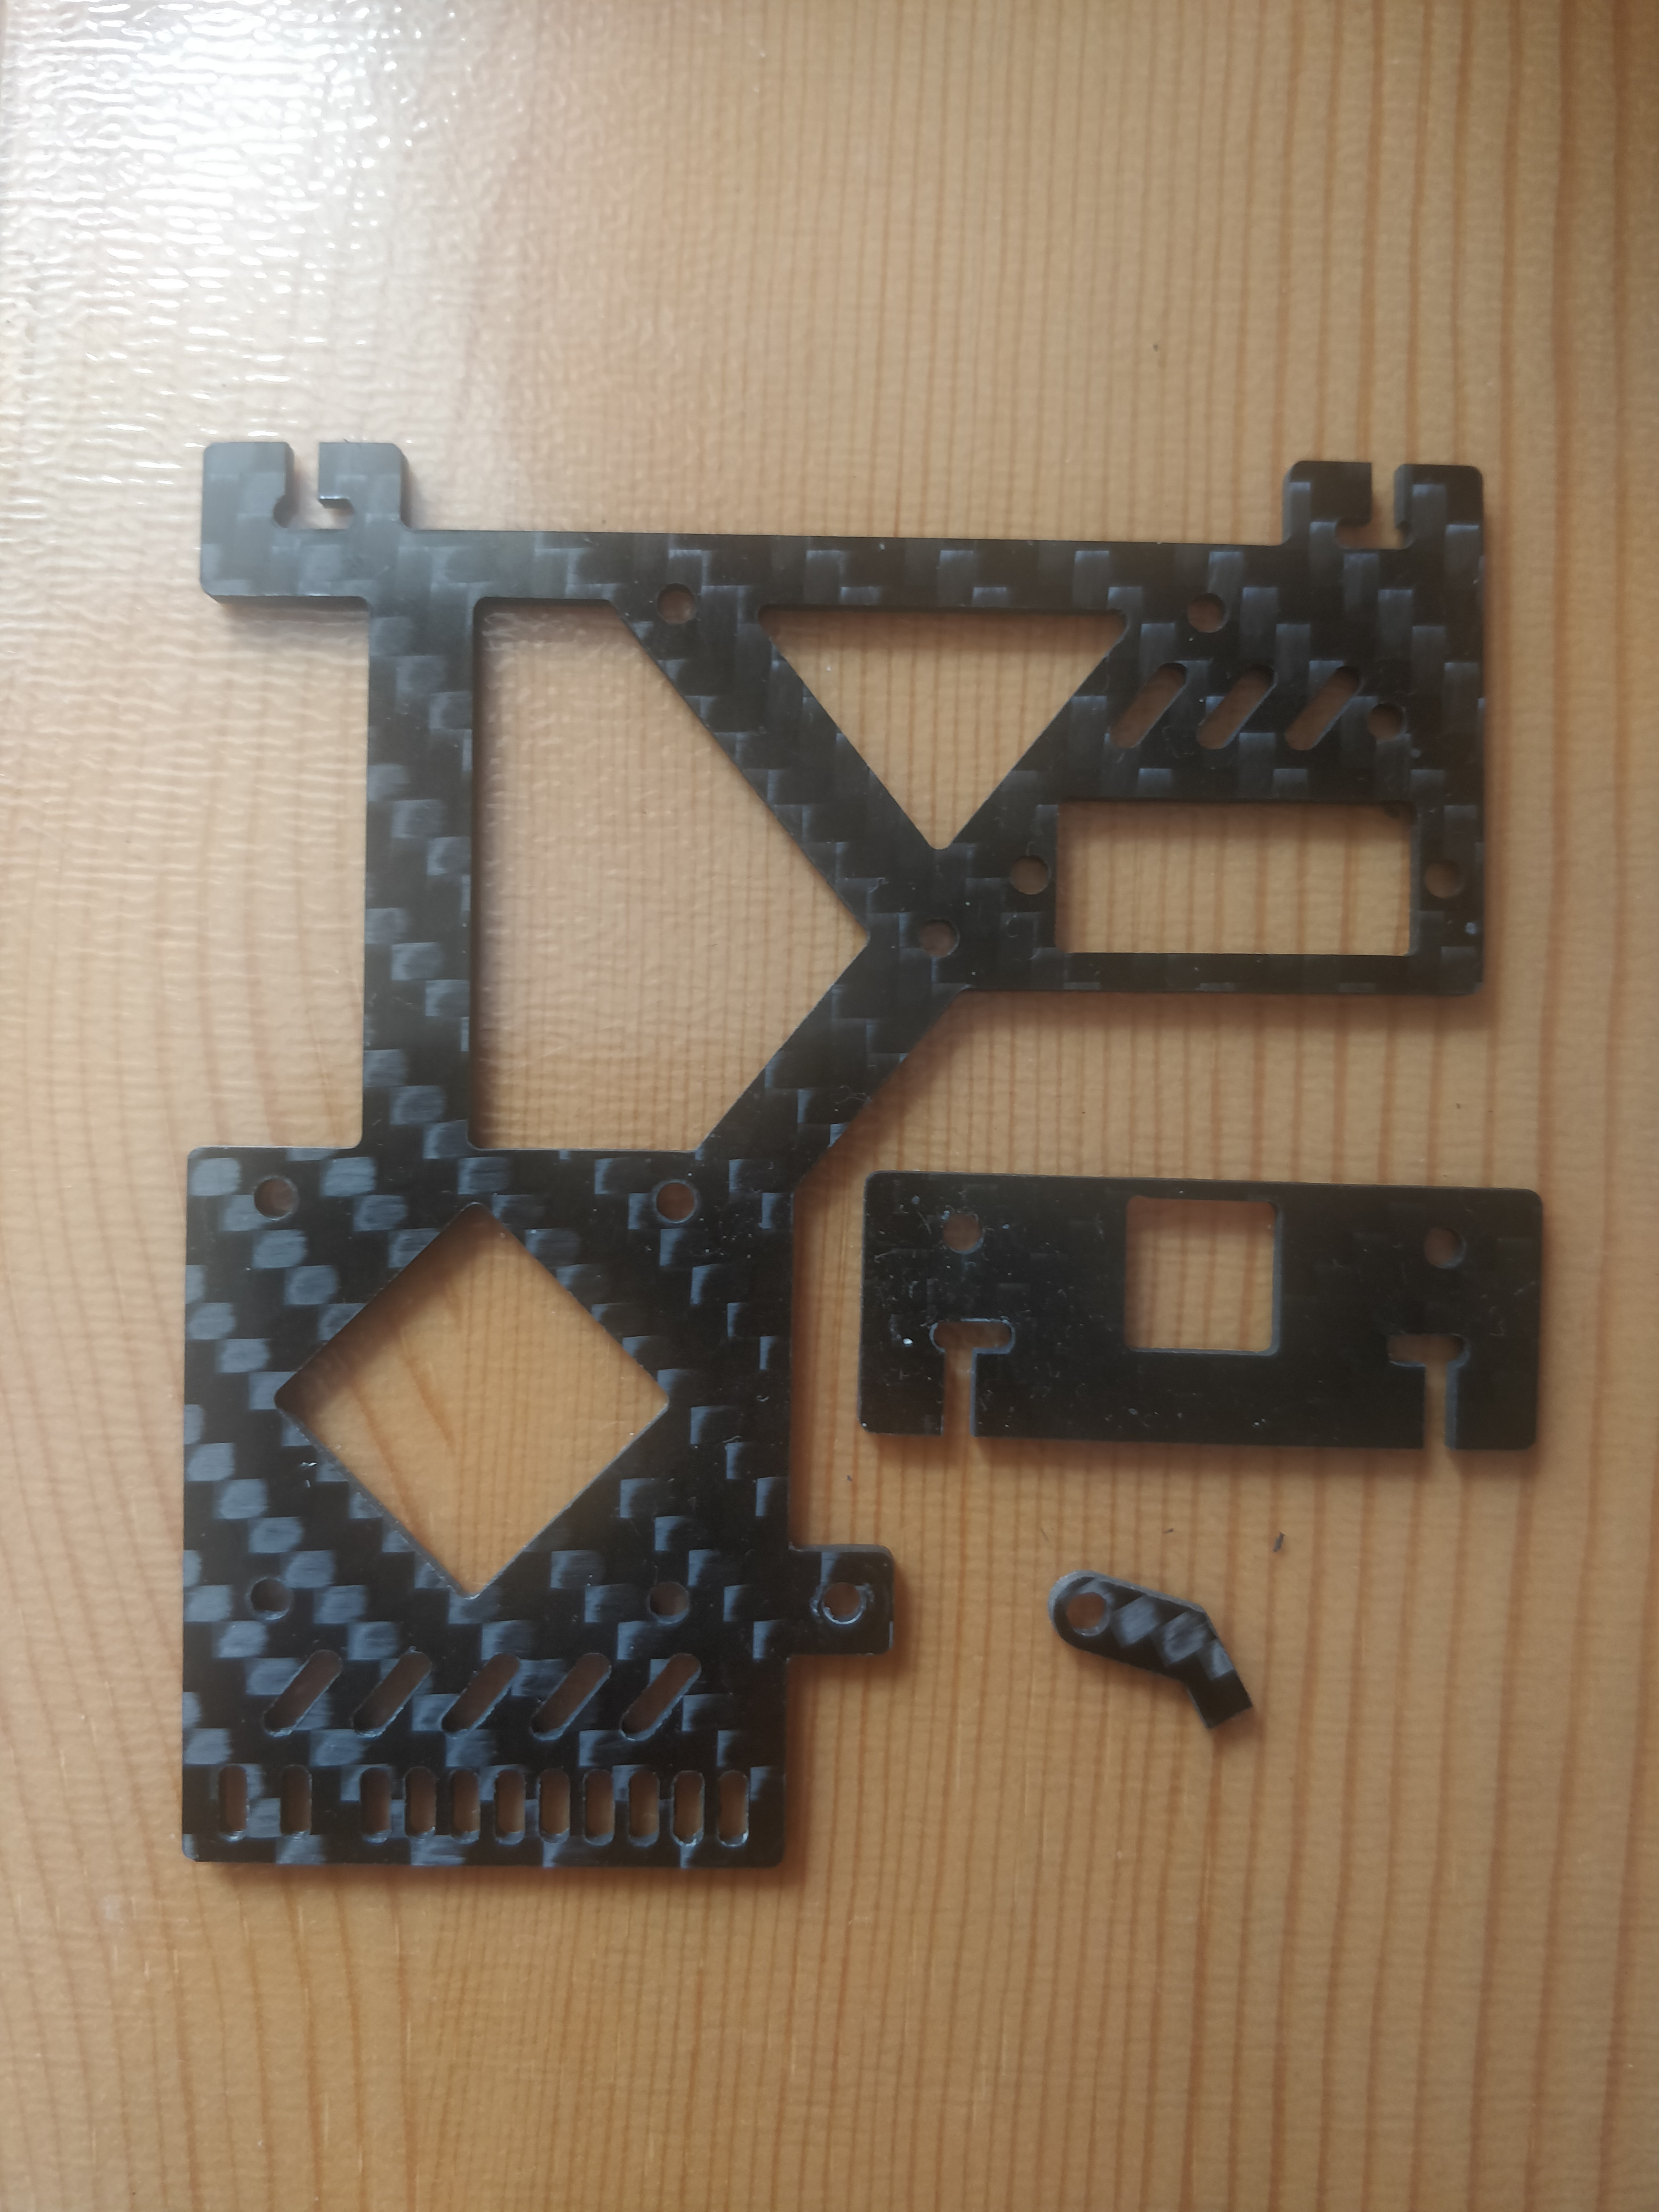
\includegraphics[height=7cm]{carbon_fiber.jpeg}
  \caption{碳纤维切割实物(部分)}
  \label{fig:carbon_fiber}
\end{figure}
机翼接头使用了3D打印ABS材质。这部分也打印了两次,第一次由于不了解选择的商家的3D打印材料的膨胀系数,打印出来的孔都小于要求,商家免费给打印了第二版。虽然第二版有一个零件的孔位依然是错的,以及这次的T型接头断掉了,但自己修修补补勉强都能用(怀疑商家是手动扩的孔)。但最大的问题出在T型接头,3D打印的材料与碳纤维杆之间的摩擦力在舵机拉动时无法忽略,换成铜轴承也无法解决,因此最终换成了内部带滚珠的直线轴承。
\begin{figure}[H]
  \centering%
  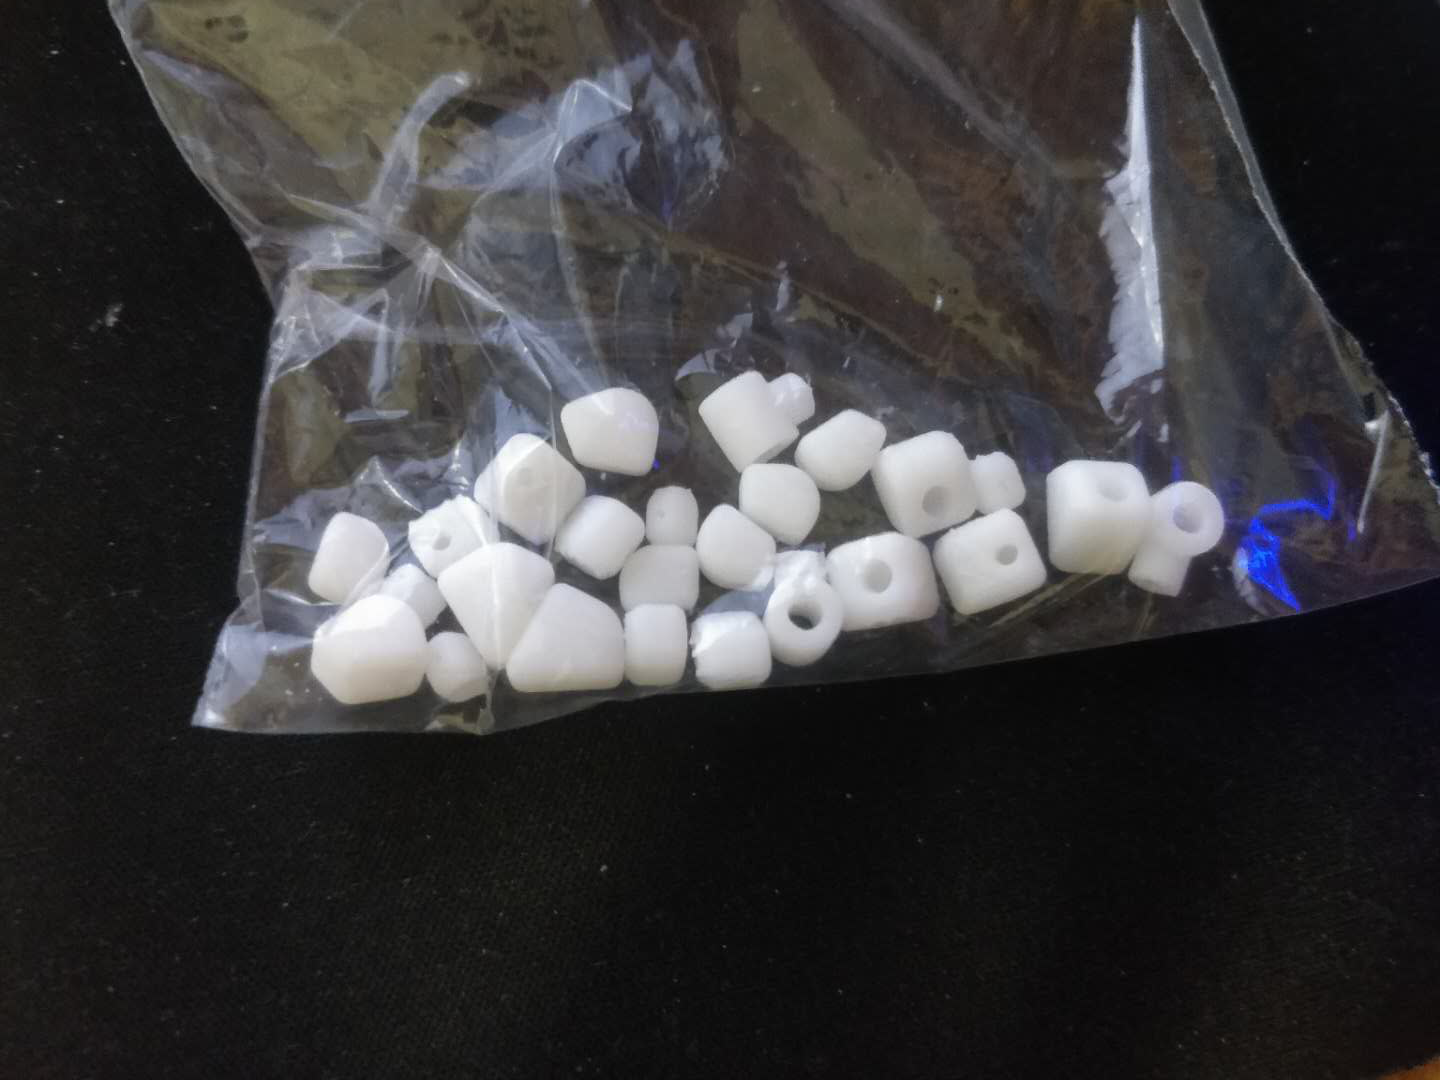
\includegraphics[height=6cm]{3Dprint.png}
  \caption{3D打印零件}
  \label{fig:3Dprint}
\end{figure}
\begin{figure}[H]
  \centering%
  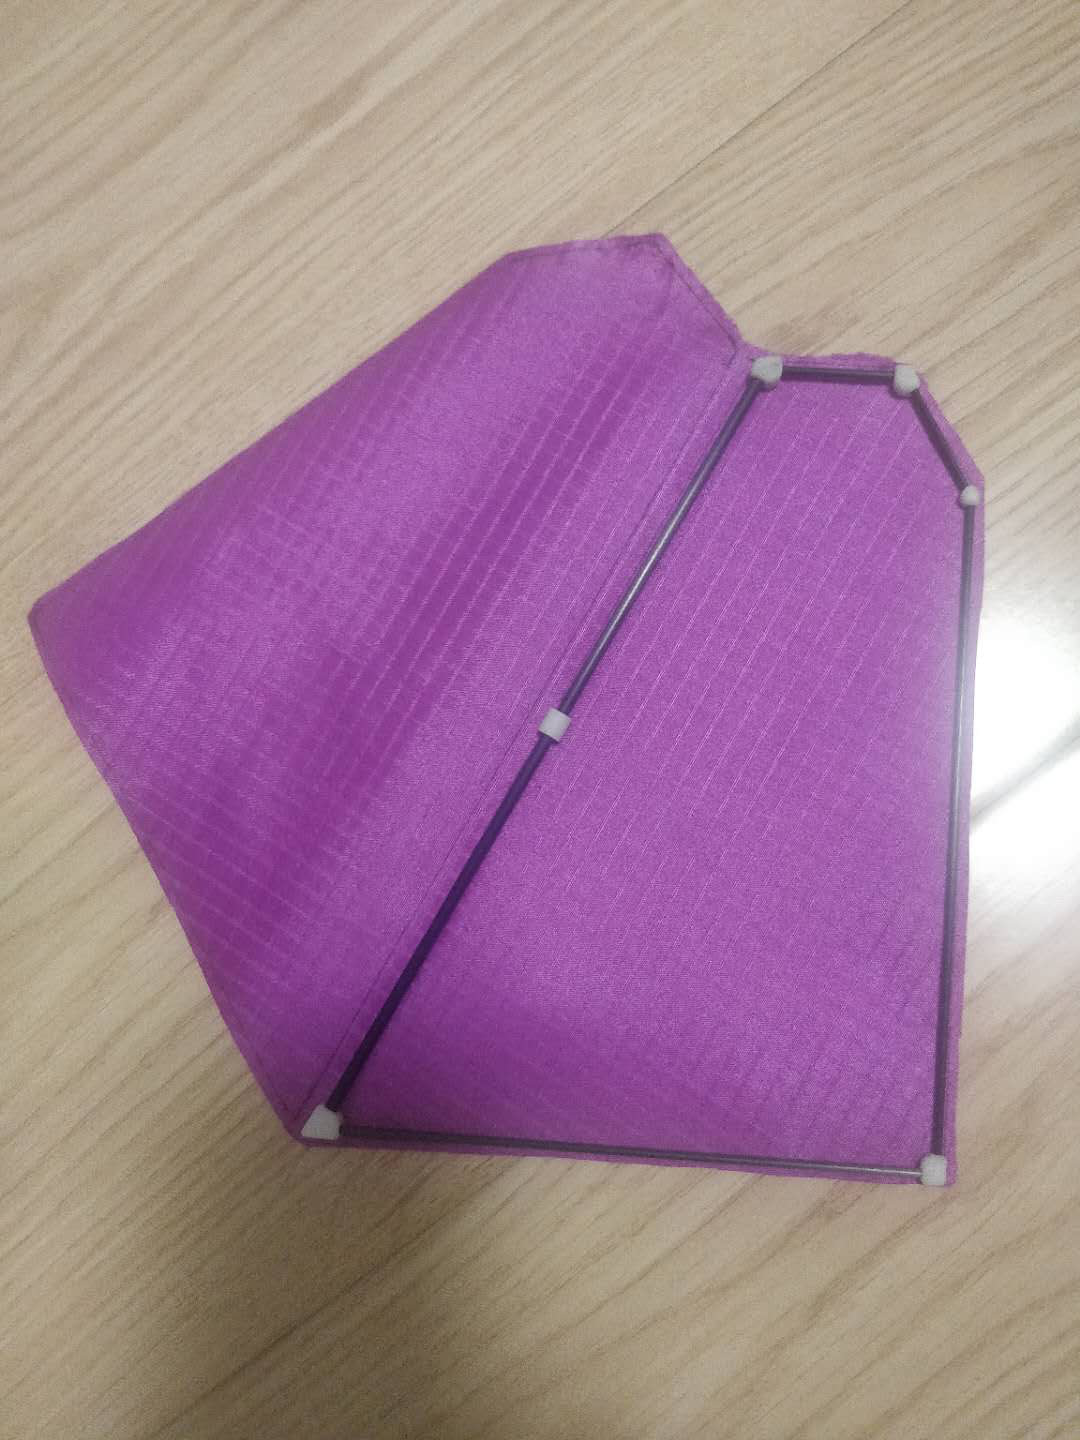
\includegraphics[height=8cm]{wing_assembled.png}
  \caption{机翼组装}
  \label{fig:wing_assembled}
\end{figure}
腿的部分最大的问题来自于元件之间连接的间隙与晃动。设计时各部分是平面设计,连接轴使用了直径2mm的碳纤维杆和金属杆,杆与板的固定使用了卡簧。而实际发现,卡簧径向的摩擦力不够可靠,而且一些关节的晃动会被机构放大,几次运动之后晃动就大到无法接受。因此使用AB胶对关节进行了加固,如图\ref{fig:leg_assembled}所示,效果拔群。
\begin{figure}[H]
  \centering%
  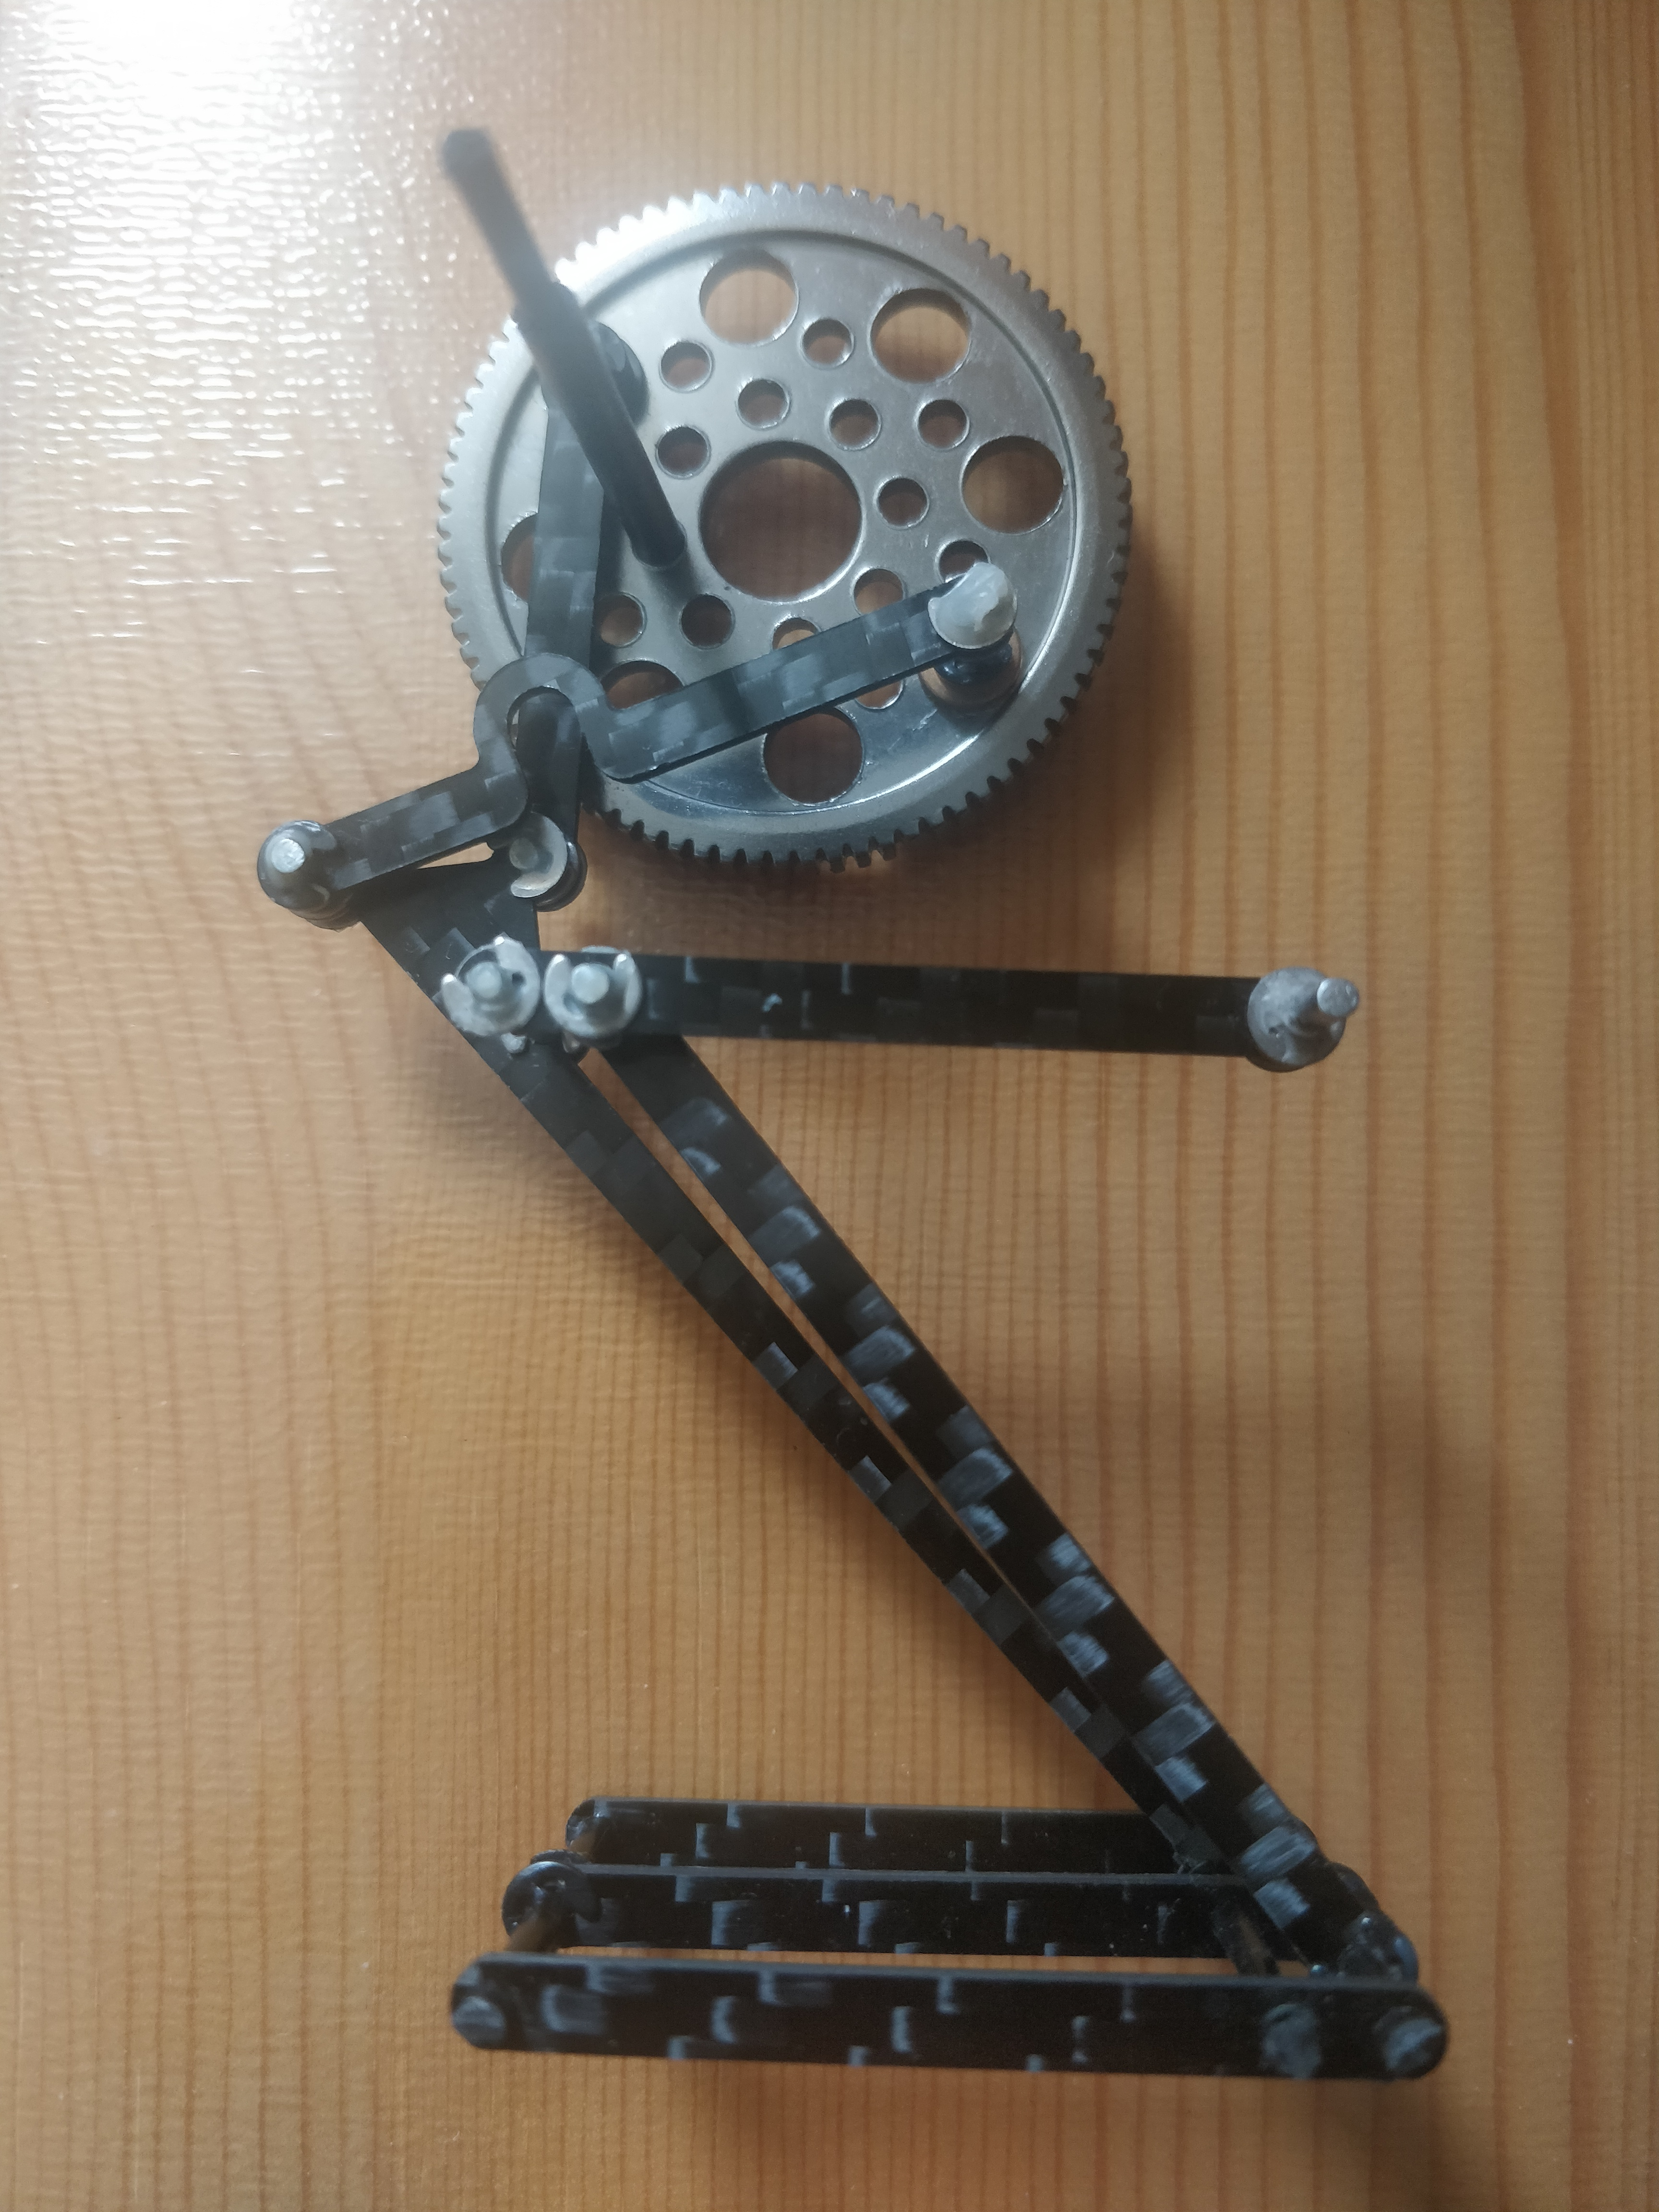
\includegraphics[height=9cm]{leg_assembled.jpeg}
  \caption{AB胶加固后的腿}
  \label{fig:leg_assembled}
\end{figure}
减速器部分同理,次级齿轮用2mm打头轴和卡簧固定,在运动一段时间后卡簧松动,轴会发生歪斜从而导致齿轮卡住。用AB胶固定后改善,如图\ref{fig:retarder_assembled}所示。
\begin{figure}[H]
  \centering%
  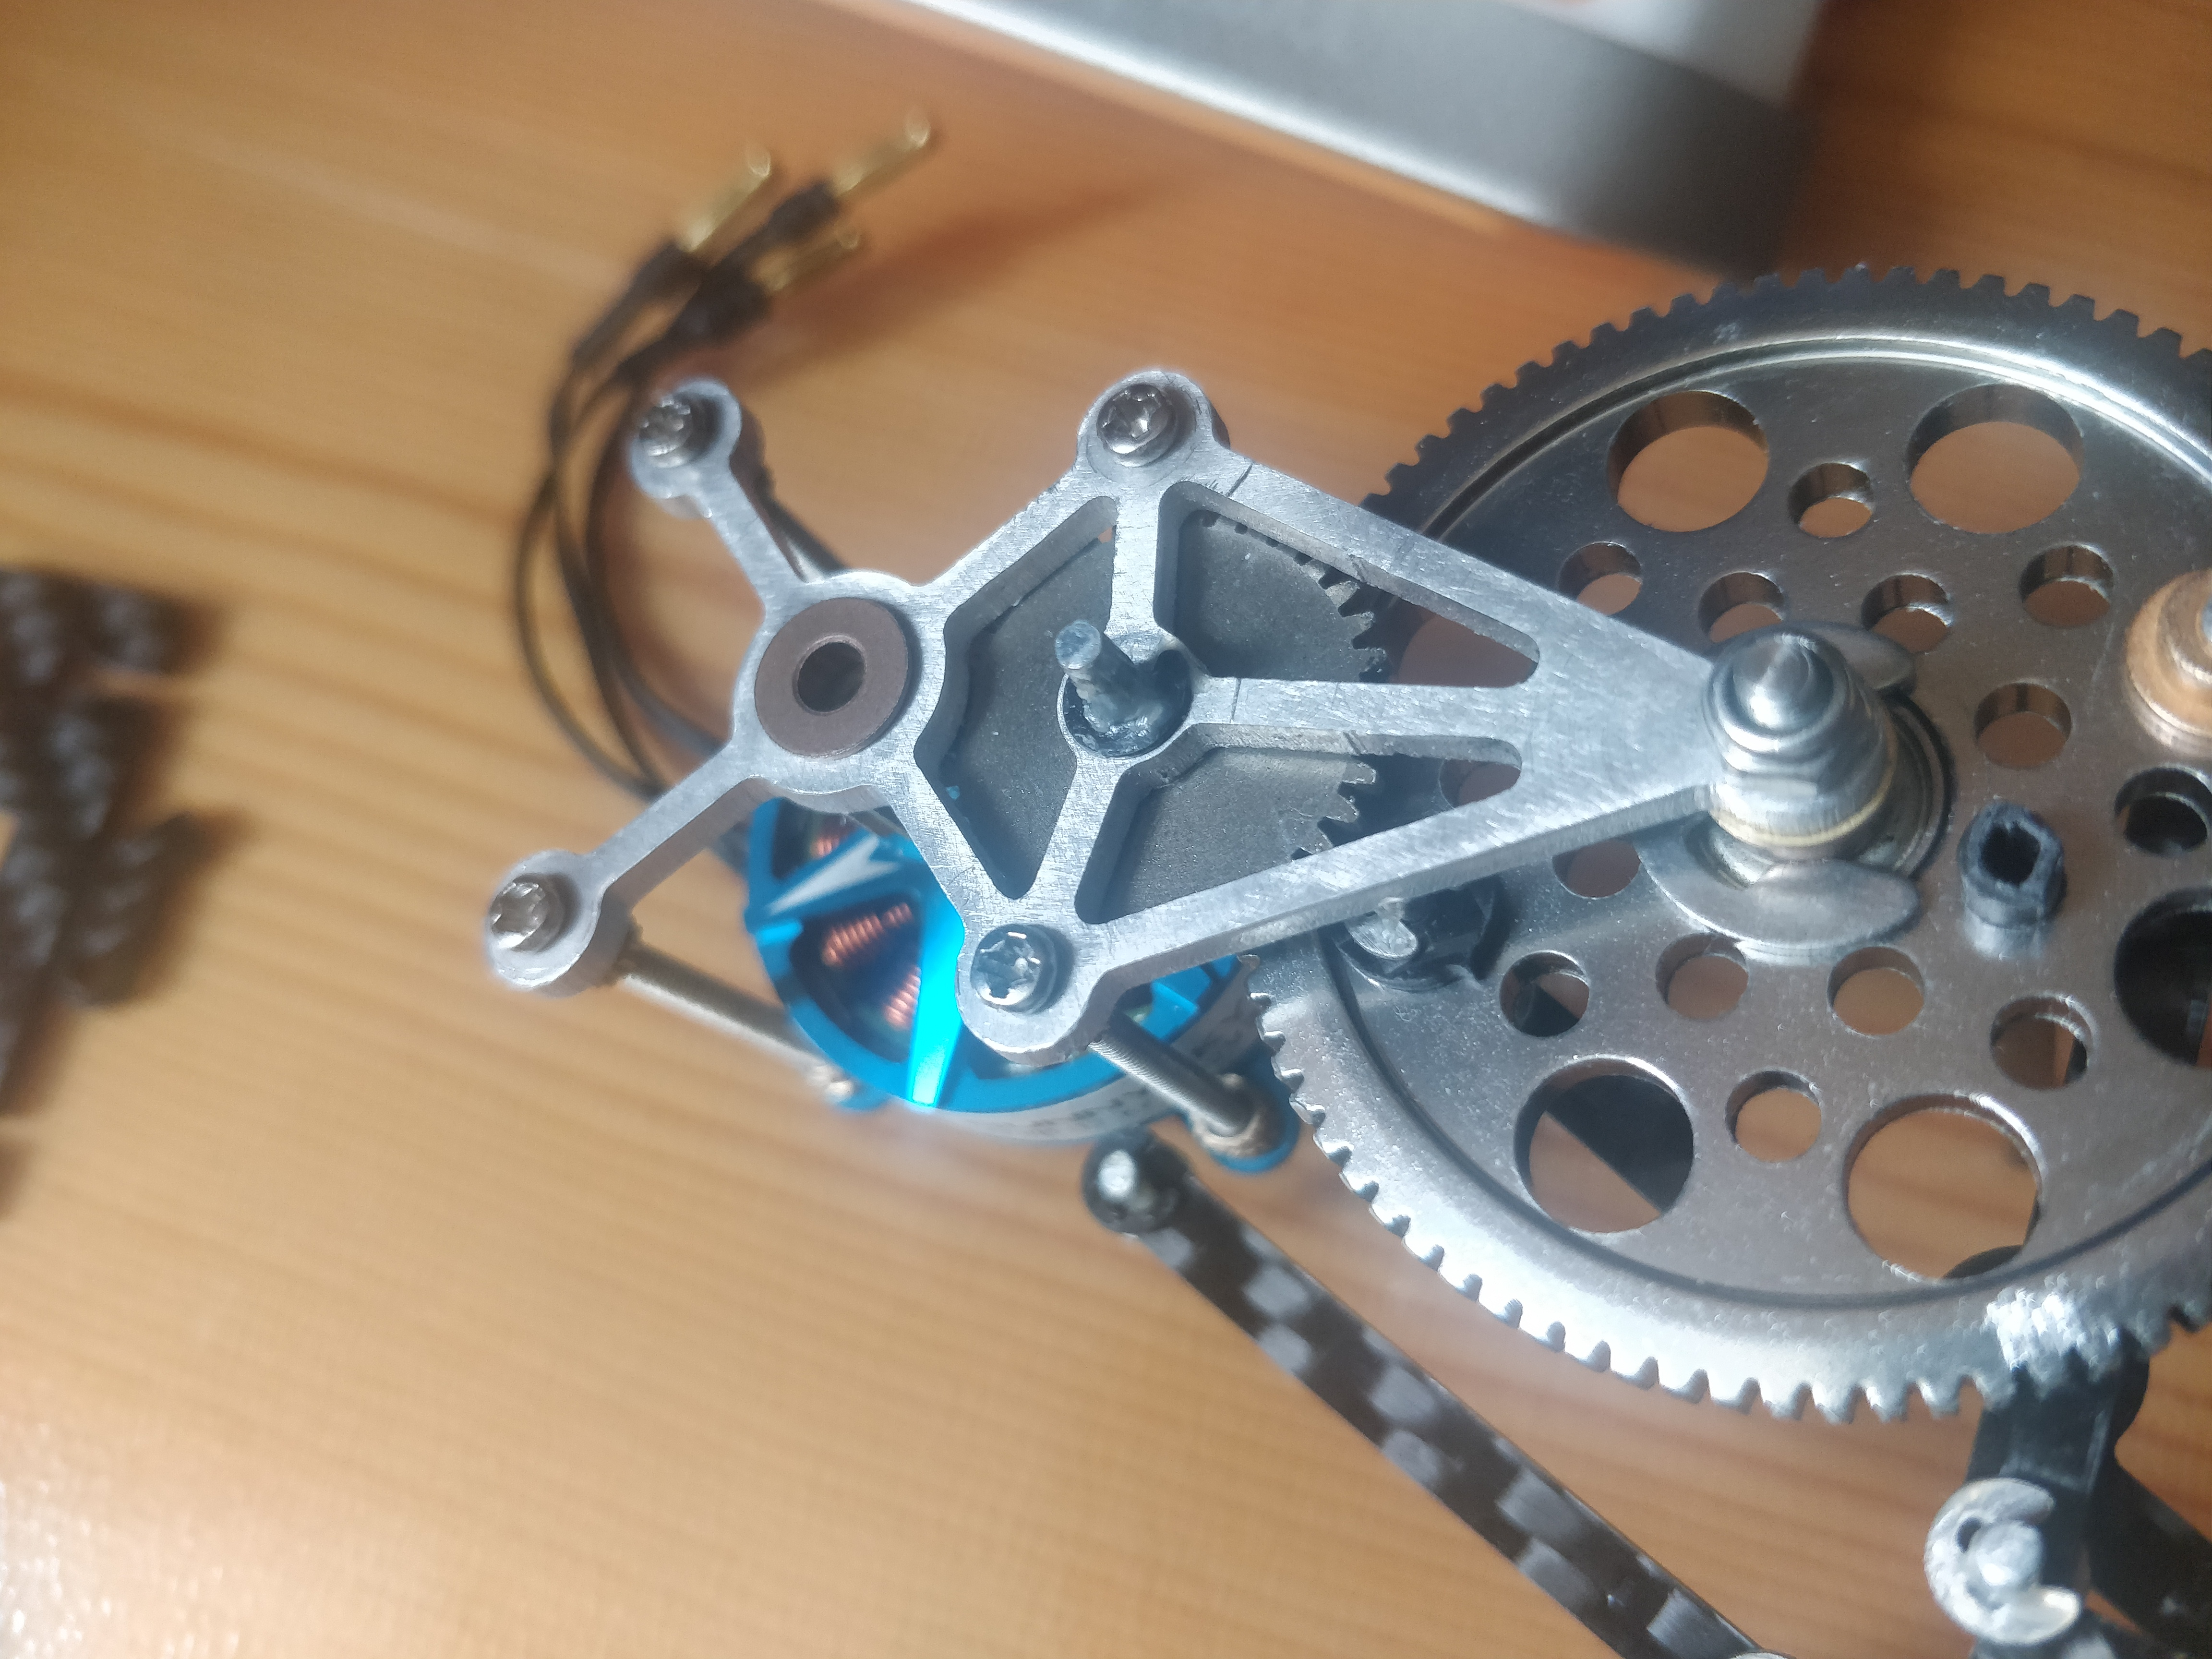
\includegraphics[height=7cm]{retarder_assembled.jpeg}
  \caption{AB胶加固后的减速器}
  \label{fig:retarder_assembled}
\end{figure}
最终组装成品图如图\ref{fig:assembled}所示:
\begin{figure}[H]
  \centering%
  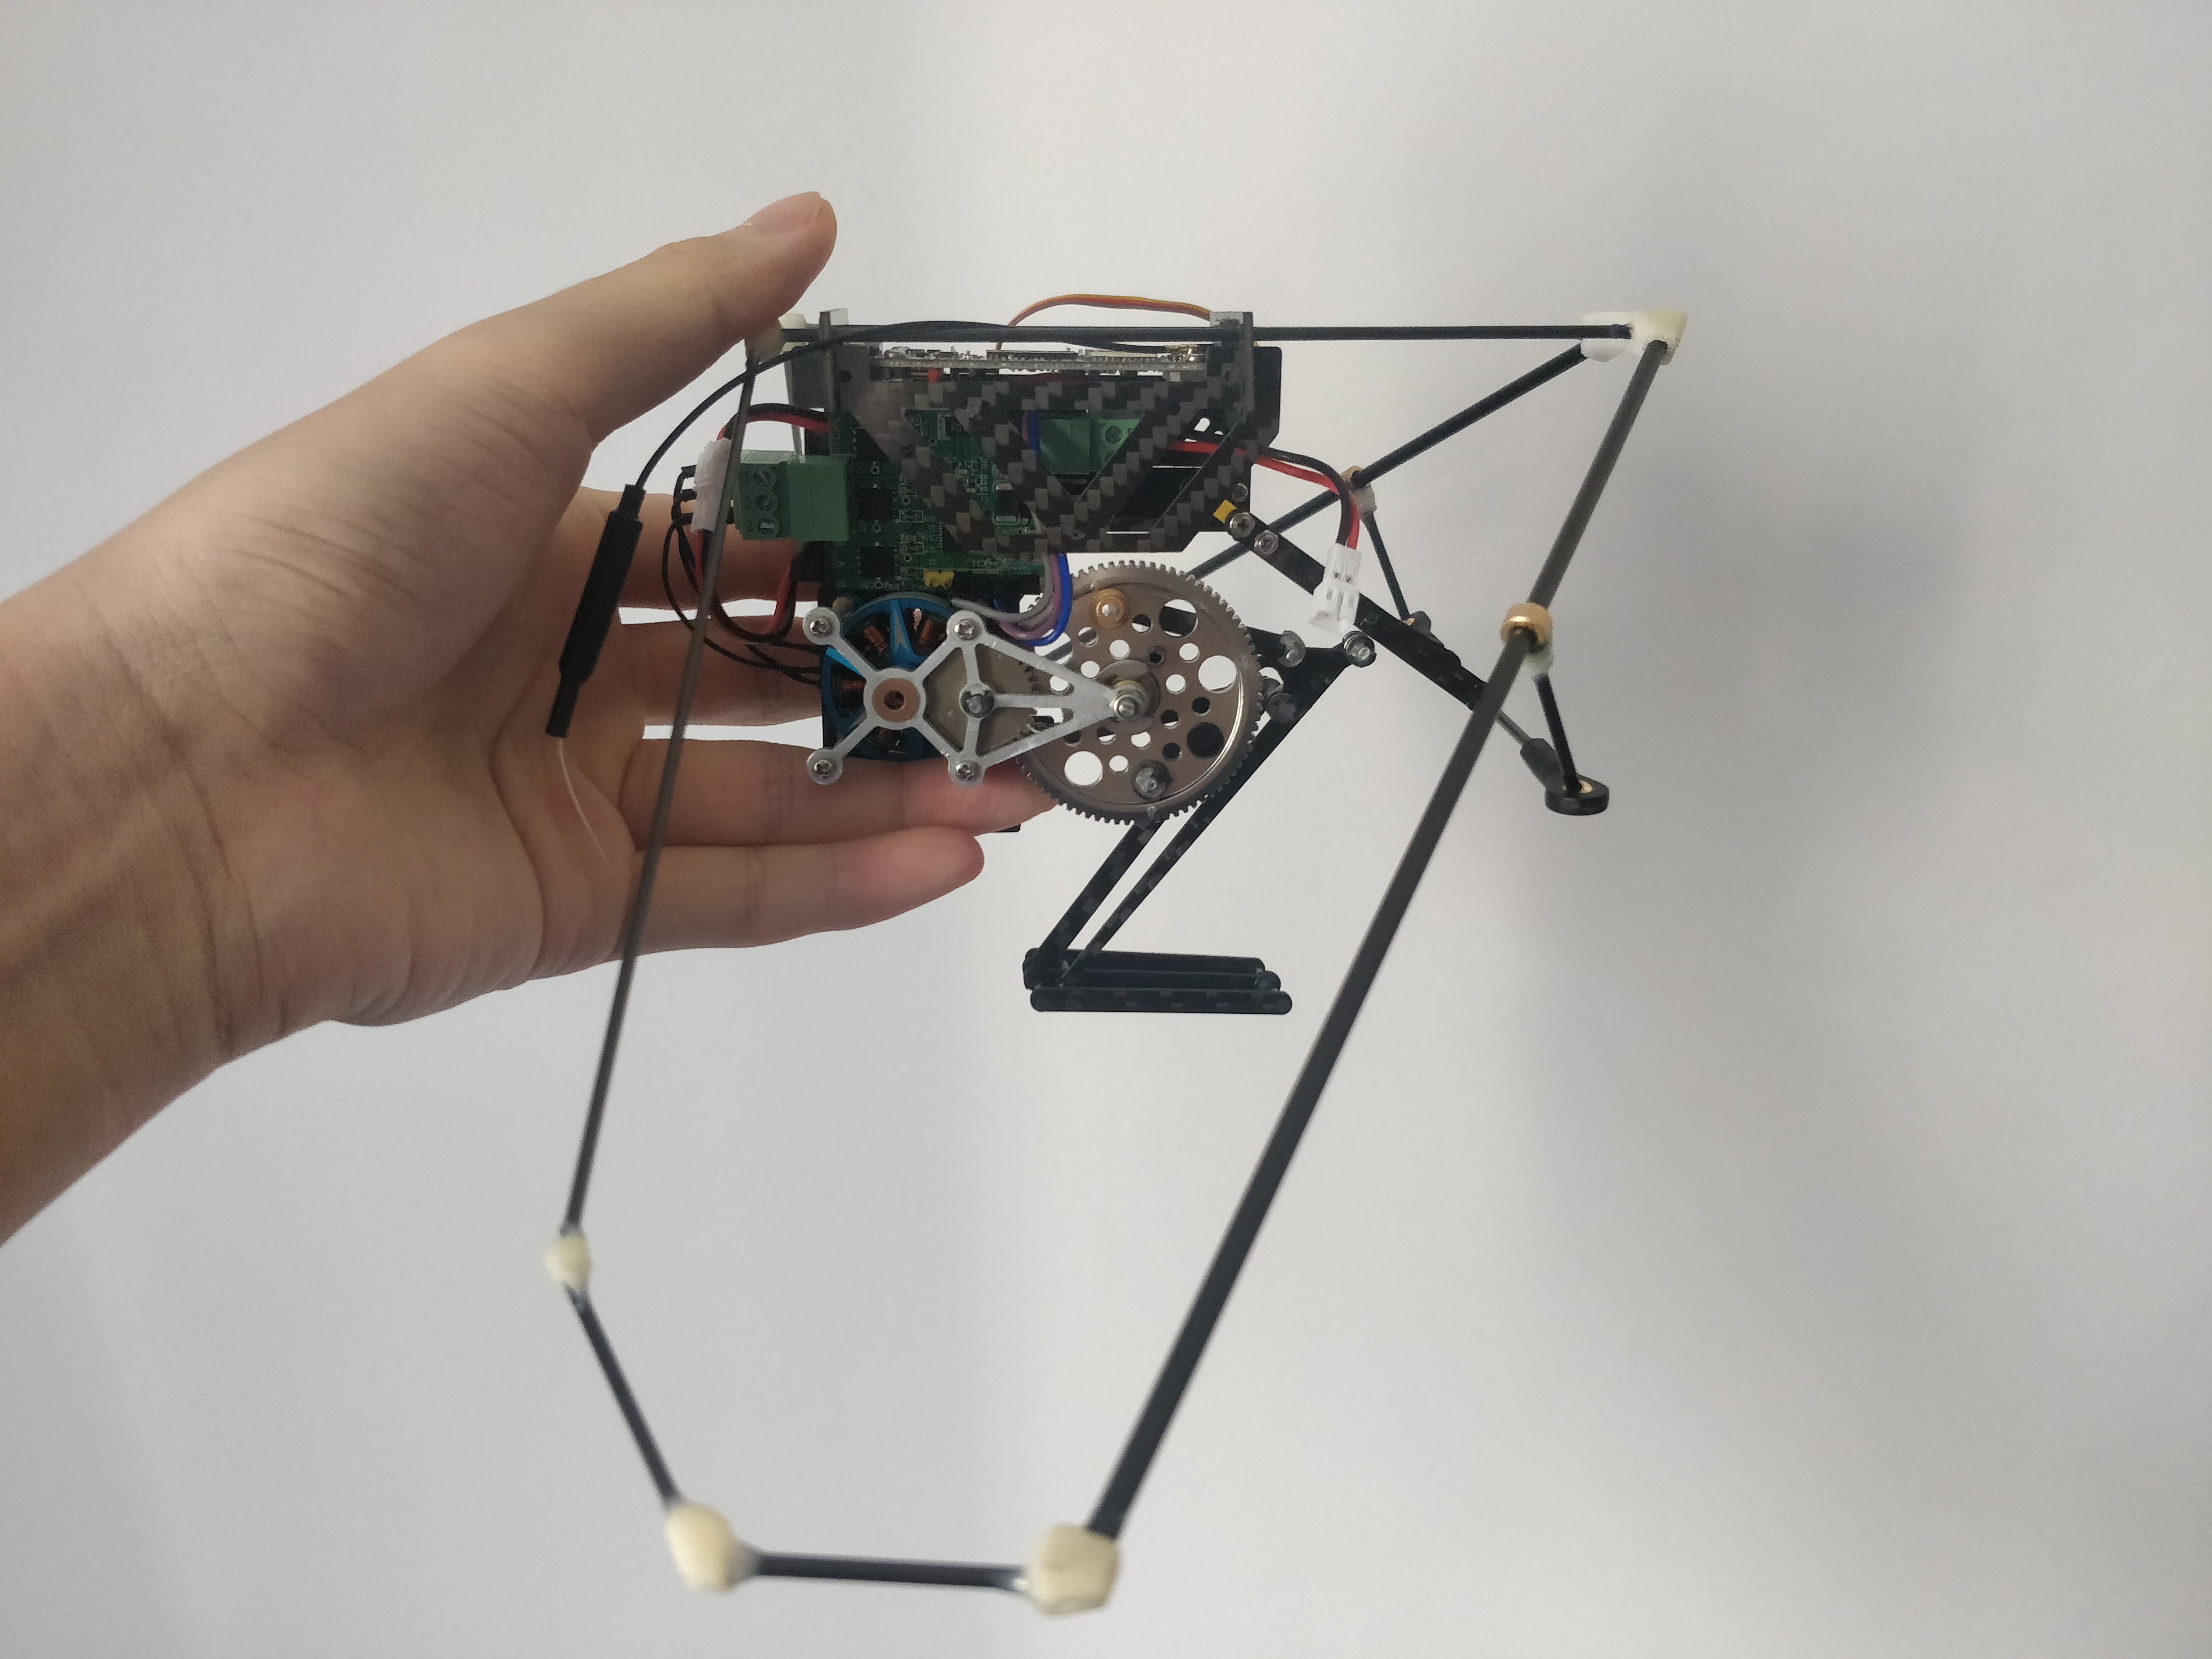
\includegraphics[height=10cm]{assembled.jpeg}
  \caption{组装成品图}
  \label{fig:assembled}
\end{figure}
\section{电机测试}
电机控制测试部分分为空载和带载测试。空载测试配置如图\ref{fig:motor_test}所示。通过改变电机启动电流曲线,进行了平稳启动(2.5s内从0加速至1000rpm)和快速启动(120ms内从0加速至10000rpm)测试,并用MotorControl Workbench自带的画图工具进行了速度监测,得到结果如图\ref{fig:motor_test_speed}所示:

\begin{figure}[H]
  \centering%
  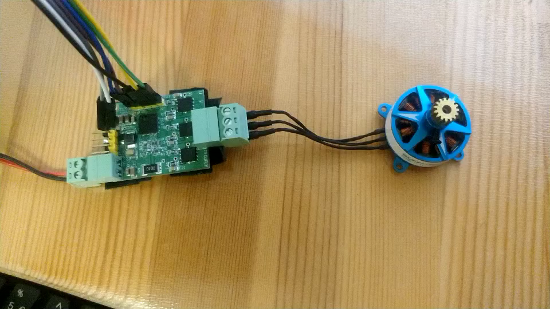
\includegraphics[height=5cm]{motor_test.png}
  \caption{空载配置}
  \label{fig:motor_test}
\end{figure}
\begin{figure}[H]
  \centering
  \subcaptionbox{平稳启动\label{fig:motorspeed1}}[6cm] 
    {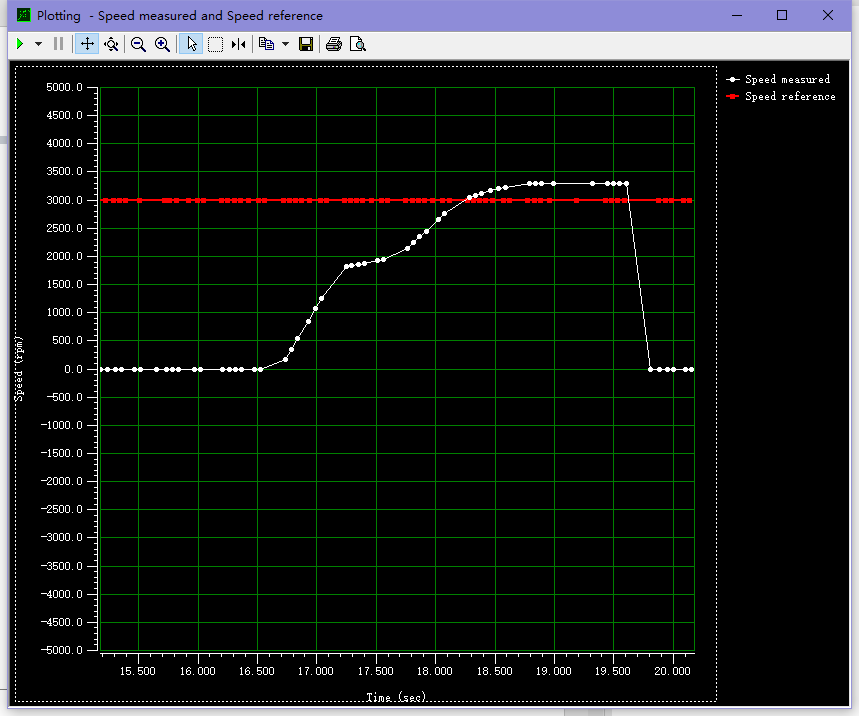
\includegraphics[height=5cm]{motorspeed1.png}}
  \hspace{4em}
  \subcaptionbox{快速启动\label{fig:motorspeed2}}
      {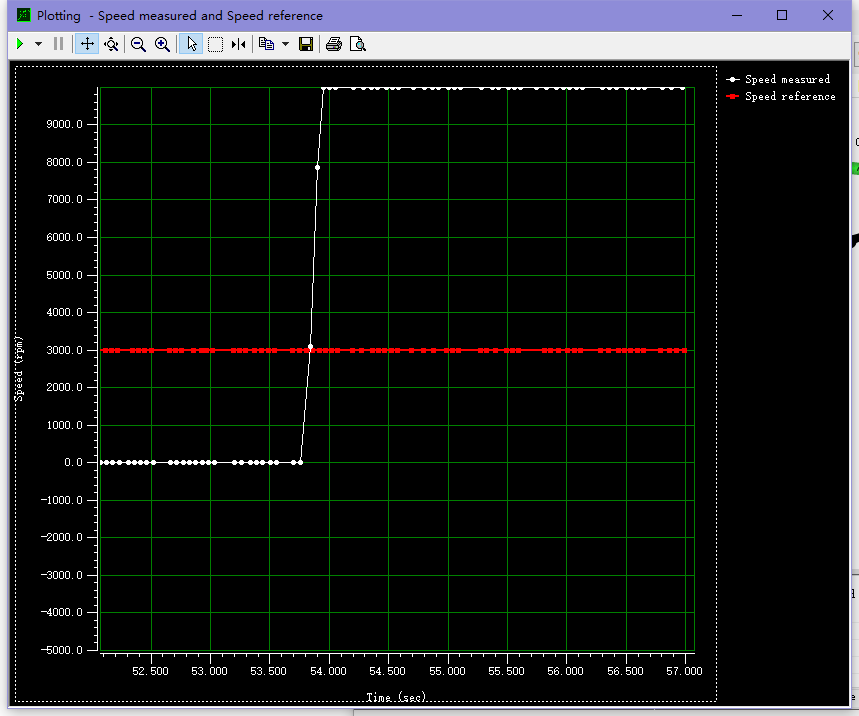
\includegraphics[height=5cm]{motorspeed2.png}}
  \caption{空载测试结果}
  \label{fig:motor_test_speed}
\end{figure}
带载测试配置如图\ref{fig:retarder_test}所示,只安装减速器便于观察输出级齿轮行程,按照同样的参数进行平稳启动和快速启动测试,结果如图\ref{fig:retarder_test_speed}:
\begin{figure}[H]
  \centering%
  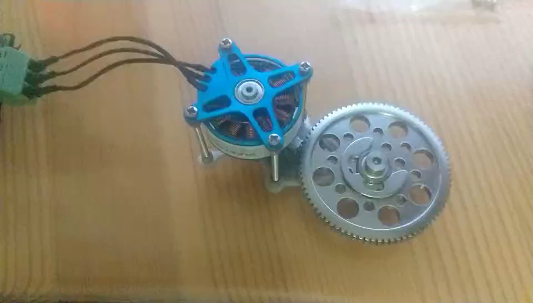
\includegraphics[height=5cm]{retarder_test.png}
  \caption{带载配置}
  \label{fig:retarder_test}
\end{figure}
\begin{figure}[H]
  \centering
  \subcaptionbox{平稳启动\label{fig:motorspeed3}}[6cm] 
    {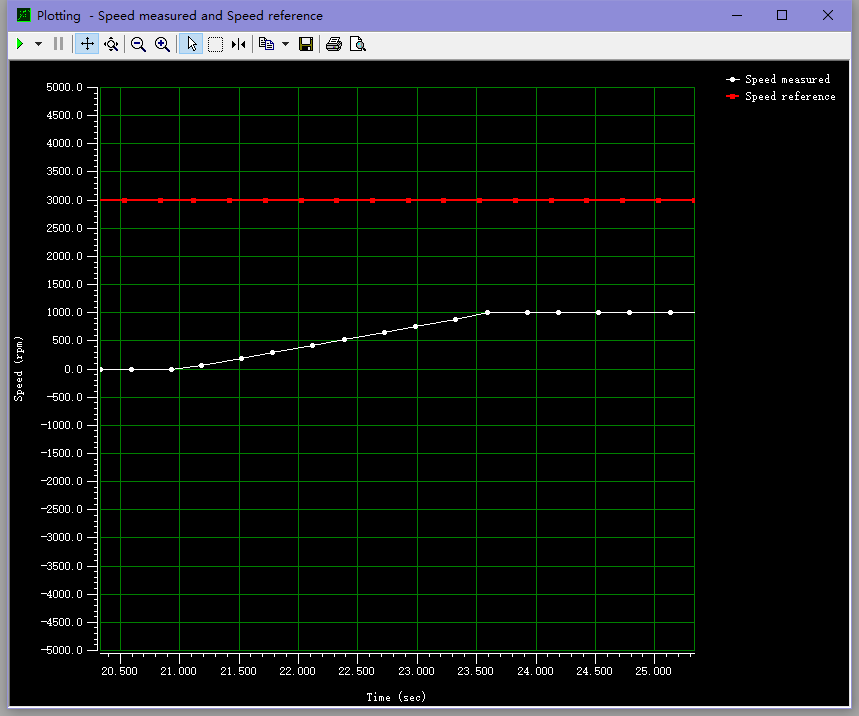
\includegraphics[height=5cm]{motorspeed3.png}}
  \hspace{4em}
  \subcaptionbox{快速启动\label{fig:motorspeed4}}
      {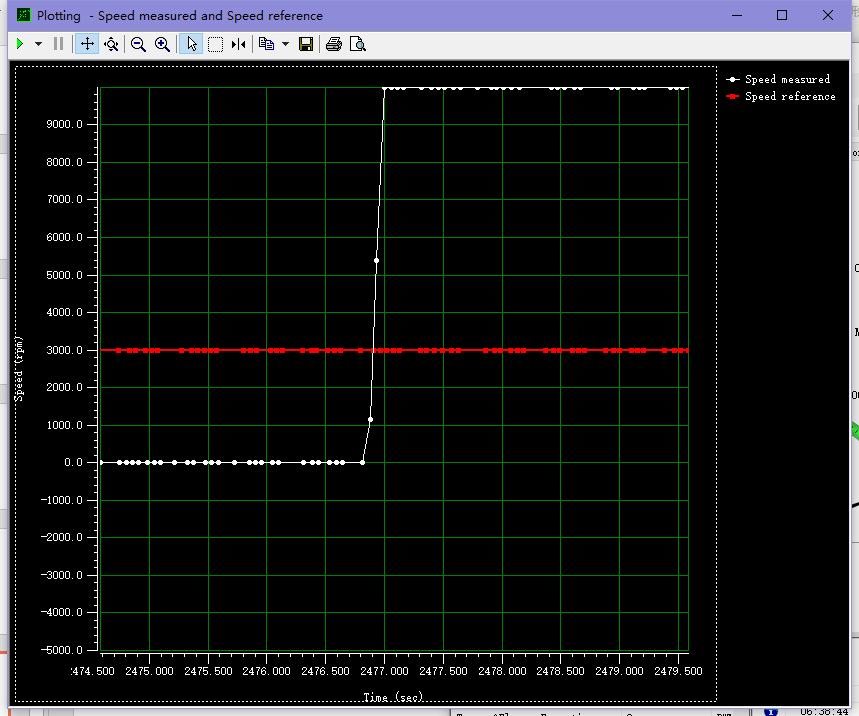
\includegraphics[height=5cm]{motorspeed4.png}}
  \caption{带载测试结果}
  \label{fig:retarder_test_speed}
\end{figure}
测试结果中横坐标为时间(s),纵坐标为转速(rpm),因此启动曲线下方到横轴的面积即为电机行程(转数)。将快速启动曲线近似成直线,则输出级齿轮行程:$$\Theta=\frac{1}{2}\omega_{max}t\div60\div i=0.52(r)$$
大致为半圈,符合设计需求。
\section{跳跃测试}
\section{机翼测试}
\section{整体测试}
\section{项目总结}